%why qec and principles here, intro to what qc are and what they can do

Quantum computers are devices that exploit the features of quantum mechanics at
the smallest scales of reality. They have the potential to solve computational
problems that cannot be solved in any reasonable time on conventional computers
\cite{fowler12_surfac_codes}. In principle, quantum computers will be able to
accurately simulate physics \cite{feynman82_simul_physic_with_comput}, or implement
algorithms, such as Shor's factoring algorithm \cite{Shor_1997}, or Grover's
search algorithm \cite{Grover_1996}, in polynomial time, providing a massive
speedup to computationally hard problems of interest. To date, superconducting
LC circuits have shown the greatest promise in forming effective quantum bits
(or qubits) \cite{Rol_2019} \cite{barends14_super_quant_circuit_at_surfac},
however several other platforms, such as quantum dots
\cite{huang19_fidel_bench_two_qubit_gates_silic} \cite{Lawrie_2020}, NV-centres
in diamond \cite{Taminiau_2014}, and even topological qubits in semi-conducting
nanowires \cite{Mourik_2012}, have seen growing interest and recent development.

Realizing a full, scalable, and reliable quantum computer is complicated by the
fact that qubits are highly susceptible to noise, be it from their environment
or through imperfections in the physical apparatuses, which will
cause qubit decoherence, losing the very information that makes them so useful.
To date, using various techniques, the upper bound on how long qubit coherence
can be extended stretches to about 1 second \cite{Abobeih_2018}, but most lose
coherence much sooner. In order for these qubits to be useful in computations,
it will be necessary to preserve their states for much longer and to correct
their states when they are subject to \textit{errors} due to environmental
noise. Quantum error correction aims to protect qubits from noise processes,
making reliable computation possible.

\subsection{Principles of Quantum Error Correction}
In the basic theory of quantum error correction, quantum states are encoded into
several physical qubits, and the states of these encoded qubits can be probed
through the measurement of stabilizers, which give information on the encoded
states without affecting their states (thanks to the non-destructive nature of
parity measurements) \cite{nielsen_chuang_2010}. If a certain physical qubit
which makes up the encoded, logical level qubit undergoes some error process,
this can be detected through the outcomes of the stabilizer measurements.
Effective encoding protocols are such that each error process gives rise to a
unique syndrome, which is just the list of stabilizer measurement outcomes,
which provides the information needed to correct the error \cite{fowler12_surfac_codes}.

\begin{figure}
  \centering
  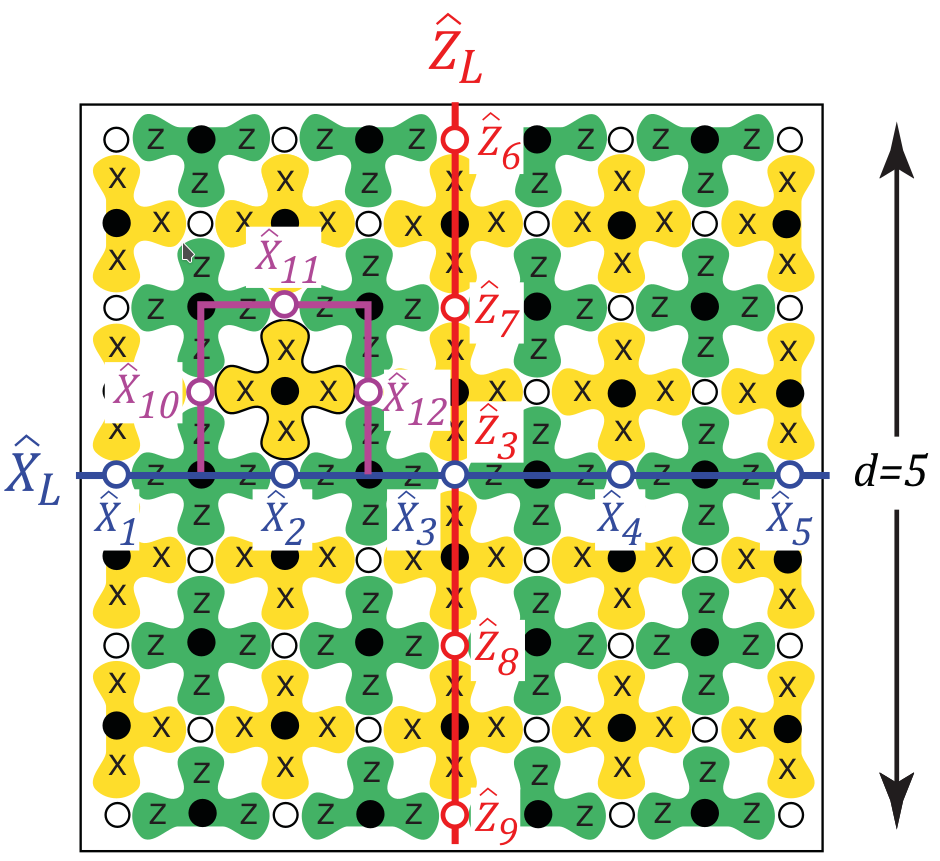
\includegraphics[width=0.4\textwidth]{images/surface_code.png}
  \caption{A 2D array of qubits implementing the surface code. Data qubits are
    the white circles, which are connected to 2 $Z$- and 2 $X$-stabilizers
    respectively. This code is capable of precisely characterizing Pauli noise
    due to the complimentary spacing of the $X$ and $Z$ checks. Figure from
    \cite{fowler12_surfac_codes}.}
  \label{fig:surface_code}
\end{figure}

In any real implementation of physical qubits, there are several sources of
error. State preparation and measurement may not be carried out perfectly, and
we can model the imperfect protocols in terms of the system having some small
chance $\epsilon$ to prepare (or measure) $|1\rangle$ when it should have
prepared (or measured) $|0\rangle$. Coherent errors also occur through the
imperfect application of quantum gates in circuits \cite{Devitt_2013}. All these
sources of error can, in principle, be corrected for using a variety of encoding
and detection schemes.

The error detection scheme implemented by the surface code, shown in Fig.
\ref{fig:surface_code}, is capable of precisely identifying errors in large
arrays of qubits. The $X$- and $Z$-stabilizer ancillas conduct parity
measurements between the data qubits to which they are connected through a
sequence of CNOT operations. Should an error occur on a given data qubit,
depending on the error type ($X$, $Y$, or $Z$) either the $X$ or $Z$ (or both) type
stabilizers will fire (return eigenvalues of $-1$), alerting us to the error. 

One great strength of the surface code is its ability to diagnose multiple
errors simultaneously. Should two adjacent $X$-checks fire at one end of the
surface, while two $Z$-check fire at the other end, we can conclude that a
phase-flip error occurred on the data qubit between the two $X$-checks, while a
bit-flip error occurred between the $Z$-checks. One must be careful, however,
because decoding the error syndrome for any code is a problem without a unique
solution \cite{terhal15}. Taking the top-left data qubit in Fig. \ref{fig:surface_code} as an
example, one can confirm that a bit-flip error on that qubit would give rise to
the exact same syndrome as a series of bit-flip errors on the rest of the top
row of data qubits. For systems with small error probabilities, the single
bit-flip error is of course much more likely than the long series of errors
required to produce the same syndrome, but as the error rate grows, such
mistakes in identifying the cause of a syndrome become more commonplace. 

When a syndrome is misinterpreted, the code implements the \textit{wrong
  correction}, and this can lead to a logical level operation being applied to
the logical qubit. A parameter of great interest in error correction codes is
this logical error rate, and specifically how it depends on and improves on the
physical error rate of the system in question. 

% One of the simplest such
% examples of error correcting codes is the \textit{repetition code}, where logical level
% qubits are encoded as,
% \begin{equation}
%   |\bar{0}\rangle = |000\rangle ,  \:\:\:\:\:\:
%   |\bar{1}\rangle = |111\rangle .
% \end{equation}
% These encoded states, along with the stabilizers $Z_1 \otimes Z_2 \otimes I_3 =
% ZZI$ and $I_1 \otimes Z_2 \otimes Z_3 = IZZ$, protect the quantum state against
% bit-flip ($X$ type) errors in the physical qubits. Operators must be promoted to
% the logical level in order to implement the right operations, allowing us to
% define $\bar{X} = XXX$ and $\bar{Z}=ZZZ$. Under normal operation, both
% stabilizers return an eigenvalue of $+1$ for the $|\bar{0}\rangle$ and
% $|\bar{1}\rangle$ states. In the presence of a bit-flip error, for example on
% the first qubit, where $|\bar{0}\rangle \rightarrow |100\rangle$, the first
% stabilizer measurement $ZZI$ will return an eigenvalue of $-1$, signalling that
% an error has occurred on the logical level bit. Even better, as long as we limit
% ourselves to single errors, the stabilizer outcomes, collectively called the
% error \textit{syndrome}, uniquely identify which physical qubit was subject to
% the error. This brings about the possibility of \textit{error correction}. We
% can probe the system to ask whether it is still in a valid logical state, and if
% not, we find from the outcome of our stabilizer measurements what the most
% likely error to have occurred is, and we can subsequently correct this.

% This simple example has several drawbacks though. It can be shown that
% certain two qubit errors give rise to the exact same syndrome as single qubit
% errors, meaning that the correction that needs to be applied is no longer
% unique, and applying the \textit{wrong} correction can in fact lead to a logical
% gate being applied to the qubits. The logical error rate of encoded qubits, as a function of the
% physical error rate, is a key parameter of interest in characterizing the
% effectiveness of an encoding protocol. Another limitation of this simple code is
% it inability to correct for phase-flip ($Z$ type) errors. Since these errors
% commute with the stabilizer group, they go undetected by the above scheme.

% There are many encoding schemes, of various sizes, that can correct for single
% bit-flip and phase-flip errors \cite{PhysRevLett.77.793} \cite{Shor_FTQEC}. In
% general, the more reliable an error correcting scheme is to be, the higher the
% number of required physical qubits. One particularly promising encoding and
% detection scheme is the Surface Code, which we will elaborate more on in the
% sections to come. 

%%% Local Variables:
%%% mode: latex
%%% TeX-master: "QEC_paper"
%%% End:
